\section{Initial Theory}
In terms of a Wireless Channel in the proposed Fall Detection System, it is preferred for the receiver to be able to estimate the state of the wireless channel. This can allow for optimisations to be made for optimal propagation of signals from transmitter to receiver. For the receiver to understand the state of the wireless channel, many models have been made which explain the properties and state of the channel.
\subsection{WLAN Channel Model}
%%%%%%%%%%%%%%%%%%%%%%%%%%%%%%%%%%%%%%%%%%%%%%%%%%%%%%%%%%%%%%%%%%%%%
A Wireless channel model describes how the amplitude and phase of a signal changes as it propagates from the transmitter to the receiver. Most important to me is the propagation model of a wireless channel and the two main propagation models are large-scale propagation known as large-scale path loss and small-scale propagation known as small-scale fading \citep{articleWLAN}. Doppler spread can also be considered. \par
To consider both of these, large-scale path loss describes the attenuation of the signal between the transmitter and receiver. In other words, it refers to the average loss in the signal's strength over a distance. Path loss for indoor environments of 5-10m between Tx \& Rx differ greatly from larger distances. It is caused by physical phenomena due to the environment such as reflection, diffraction, absorption and many more. As the physical environment constrains the wireless signals, the received signals conveys information that represents the environment that they pass through. It is clear that as the distance between transmitter and receiver is increased, the signal and thus, signal power, is spread over a larger area suffering greater attenuation. Small scale fading occurs due to the scattering environment between the transmitter and receiver caused by obstacles in the environment. It occurs when this scattering environment changes with time \citep{articleWLAN}. This leads to the transmitted signals scattering around the environment and arriving at the receiver whereby they are added constructively or destructively, as a function of time. This demonstrates the phase-shift in the wireless channel caused by the scattering environment. The signal level changes are called fading and has two types: microscopic \& macroscopic \citep{channelModels}\par
The scattering environment is composed of Line-of-Sight (LOS) and No-Line-of-Sight (NLOS) paths introduced by various factors such as furniture, walls, ceilings and more importantly in my case, people. Under a MIMO (Multi Input-Multi Output) system with multiple transmit and receive antennas, these effects due to the scattering environment are amplified. This is what is known as utilising the spatial diversity of the channel by sending symbols on different streams/links between one transmit antenna and one receive antenna. In reference to LOS and NLOS paths, a transmitted symbol through the LOS path will clearly arrive at the receiver before the corresponding symbol through a NLOS path (See Figure \ref{fig:LOS_NLOS}). Microscopic fading occurs when the receiver receives many copies of the signal due to scattering near the receiver while Macroscopic fading occurs receives multiple delayed copies of the signal due to the scattering environment over a large distance and time period (frequency selective fading). This is characterised by the delay spread of a channel which estimates earliest and latest arrival time of significant copies of the transmitted symbol \citep{channelModels, articleWLAN}  \par
As small-scale fading is a phenomenon when the scattering signal environment changes with time for smaller changes in the distance and multiple copies of the signal arriving at the receiver at once, it will be much more useful for this project. Transmitting distances are not long enough for large-scale path loss affect signal power greatly. \par
\begin{figure}[h]
\begin{center}
  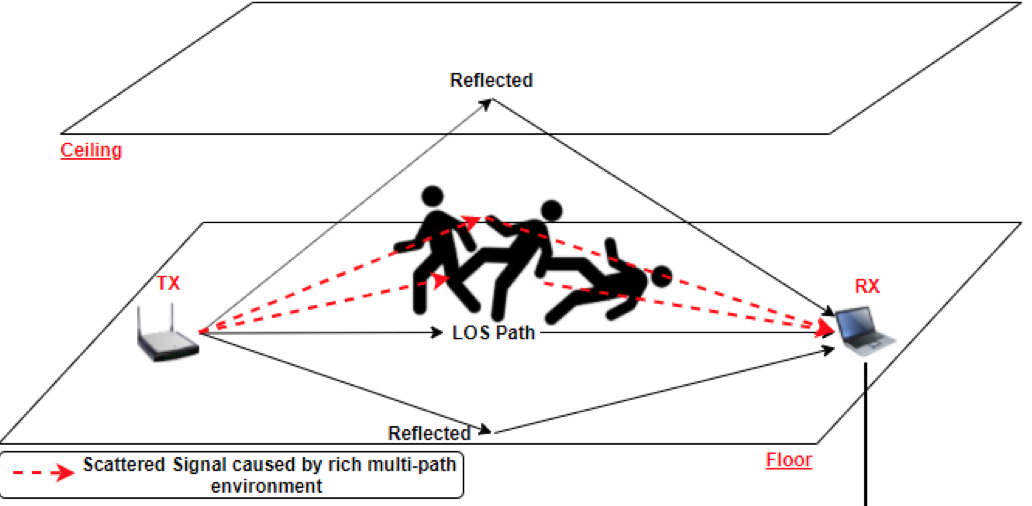
\includegraphics[scale=0.75]{Figures/Reflection.png}
\end{center}
  \caption{Demonstrates the LOS and NLOS paths between the Transmit and Receive antennas in a MIMO system. Note how the scattering environment is created due to the environment structure (floors, ceiling) and the person walking give rise to the phenomena of path loss and signal fading as discussed. Over a short LOS path, small-scale fading characterises the received signal and environment. (Diagram is taken from my Interim Presentation)}
  \vspace{-10pt}
  \label{fig:LOS_NLOS}
\end{figure}
A \textit{M} x \textit{N} (\textit{M} transmit and \textit{N} receive antennas) MIMO system can be modelled by the following equation at the receive antenna by a spatial vector \textbf{y} with a sampling period of T = 1/Bandwidth:
\vspace{-11pt}
\begin{equation}\label{eqn:2.1}
    \textbf{y}(t) = \textbf{H}(t)\textbf{x}(t)+\textbf{n}(t)
    \vspace{-11pt}
\end{equation}
where  $\textbf{x}(t) = \begin{bsmallmatrix}x_1(t) & \cdots & x_M(t)\end{bsmallmatrix}^T$ is the vector of transmitted signals, $\textbf{n}(t) = \begin{bsmallmatrix}n_1(t) & \cdots & n_N(t)\end{bsmallmatrix}^T$ is the AWGN (noise) vector for the channel and as mentioned before, $\textbf{H}(t)$ is the channel response matrix for the MIMO system at each time instance given by $t$ \citep{channelEquations}. \par
The majority of today's Wi-Fi networks operate in the 2-5GHz range and as a result, suffer from the propagation losses mentioned already of multi-path fading and path loss. Orthogonal Frequency Division Multiplexing (OFDM) was proposed to offer a robust solution at these frequencies to narrow-band interference. OFDM is the method of digital modulation whereby the signal to be transmitted is split into a number of narrow-band channels at frequencies above and below the centre frequency (5GHz for example) \citep{OFDM}.
These narrow-band channels at different frequencies are also known as subcarriers and as previously mentioned, the method to obtain higher data rates was MIMO-OFDM whereby multiple data streams are utilised between a number of transmit and receive antennas \citep{802.11nStandard}. OFDM uses a number of modulation schemes such as QAM and PSK. For each OFDM symbol, there are a number of QAM values depending on the bandwidth of the channel. The application of the IFFT modulates the OFDM symbol onto a number of subcarriers. This is followed by adding cyclic prefix to make the signal robust to multipath propagation while windowing and IQ modulation are applied before transmitting \citep{OFDM, 802.11nStandard}. \par
In Equation \ref{eqn:2.1}, the channel model for a MIMO system is described for \textit{M} transmit and \textit{N} receive antennas. However, in a MIMO-OFDM system there are a number of subcarriers depending on the bandwidth. In 802.11n, the number of subcarriers sent is dependent on the bandwidth and the grouping constant. The grouping constant is used to group adjacent subcarriers and report them as a single value to reduce the size of the report field \citep{full802.11nStandard}. Thus, Equation \ref{eqn:2.1} can be rewritten as the following for the subcarrier $k$ at one time instance for a MIMO-OFDM system:
\vspace{-11pt}
\begin{equation}\label{eqn:2.2}
    \textbf{y}_k = \textbf{H}_k\textbf{x}_k+\textbf{n}_k
    \vspace{-11pt}
\end{equation}
where $\textbf{x}_k = \begin{bsmallmatrix}x_{k,1} & \cdots & x_{k,M}\end{bsmallmatrix}^T$ is the vector of transmitted signals, $\textbf{n}_k = \begin{bsmallmatrix}n_{k,1} & \cdots & n_{k,N}\end{bsmallmatrix}^T$ is the AWGN (noise) vector for the channel. However, the channel matrix $\textbf{H}_{k}$ can be used to describe the channel response for each transmitter-receiver pair: 
\vspace{-11pt}
\begin{equation}\label{eqn:2.3}
\textbf{h}_{k}=\left[
\begin{array}{ccc}
    h_{k,11} & \cdots & h_{k,M1} \\
   \vdots & \ddots & \vdots \\
    h_{k,1N} & \cdots & h_{k,MN}
\end{array}
\right]
\end{equation}
As there are many subcarriers, there are many of these matrices $\textbf{h}_{k}$. As described by the 802.11n standard, there are 56 pilot and data sub-carriers for 20MHz bandwidth and 114 for 40MHz bandwidth with a grouping constant $N_g = 1$. These are essential to the understanding of CSI which is concerned with obtaining the Channel Impulse Response \textbf{H} seen in the next section \citep{full802.11nStandard}.
\textbf{Diagram of MIMO network and also subcarriers around the centre frequency}

\subsection{Channel State Information (CSI)}
The Channel State Information (CSI) describes the Channel Matrix \textbf{H} and thus, the wireless MIMO-OFDM channel itself. It can be described in 3-D matrix form for one packet with \textit{M} transmit antennas, \textit{N} receive antennas for a transmitter-receiver pair(Tx antenna $i$ and Rx antenna $j$)

\textbf{Diagram of the CSI matrix}

The depth of the 3-D matrix as shown above is clearly dependent on the number of subcarriers. Each subcarrier $k$ for a given transmitter-receiver pair ($ij$) conveys the channel amplitude/gain and the phase response of the channel at that time instance, $h_{k,ij} = |h_{k,ij}|e^{j\theta}$ \citep{OFDM}. Any change in the channel introduced by either path loss or multi-path fading (See Figure \ref{fig:LOS_NLOS}) will result in Channel Distortion (Amplitude distortion and phase shift).\par 
%%%%%%%%%%%%%%%%%%%%%%%%%%%%%%%%%%%%%%%%%%%%%%%%%%%
COTS Wi-Fi devices do not collect CSI data readily available for the user of the Wi-Fi NIC. However, with the arrival of the 802.11n WLAN Standard in 2009, transmit beamforming was able to be utilised which could be used to estimate the channel over which a beamformee (Rx) and beamformer (Tx) are communicating. It estimates the channel through 2 methods: Implicit feedback and Explicit feedback. In implicit feedback the beamformer receives long trained symbols from the beamformee which it uses to estimate the channel. In explicit feedback, the beamformee makes a direct estimate from the training symbols sent by the beamformer \citep{full802.11nStandard}. In other words, the goal is to focus energy towards the receiver to increase the SNR of the wireless channel \citep{beamforming}. This simply means the beamformer can adjust and maximise the signal power at the receiver depending on the current state of the channel. In a LOS scenario, it can simply be seen as the Tx forming a beam to the Rx directly. \citep{beamforming}. This can give great insight into the changing environment between Tx and Rx. \par
Currently, only Intel and Atheros Wi-Fi NICs can return CSI data through open source tools developed by a number of groups \citep{Halperin_csitool} (Intel NICs) \& \citep{Xie:2015:PPD:2789168.2790124} (Atheros NICs). The CSI of every subcarrier in a MIMO-OFDM Wireless channel is presented as a complex number $a+bj$. The CSI matrix will be of the dimensions $M$x$N$x56 for a 20MHz bandwidth and $M$x$N$x114 for 40MHz bandwidth in theory. However in practice, a Wi-Fi NIC uses several bits to represent $a$ \& $b$ (10 bits for each in Atheros NIC and 8 bits in an Intel NIC) \citep{Xie:2015:PPD:2789168.2790124}. This allows the channel to be represented in a number of complex number at a range of subcarrier frequencies. Due to transmit beamforming, we can obtain an accurate of the channel and thus, the surrounding environment. This makes it extremely useful for fall detection, activity detection and indoor localisation where there is a fixed distance between transmitter and receiver. The scattering multi-path environment introduced by an individual will be reported by each data packet's CSI matrix between Tx and Rx and thus, we can classify the activity or the environment's characteristics. This will be useful for my project for when an individual enters a room, falls, creating a large multi-path scattering environment which will be seen in the CSI data (See Figure \ref{fig:LOS_NLOS}).


\textbf{Can talk about RSSI in the related work section. Some of these do not return in base units so they use the tool which returns in absolute units with AGC added which is da da da da . Talk about how it has been used in indoor localisation, gesture recognition and others and could be used in the thing of all detection as make reference to my diagram because it scatters and suffers from multipath fading and path loss and this will be shown in CSI data at the end corresponding to a movement and then Machine learning can be used for other things}
%%%%%%%%%%%%%%%%%%%%%%%%%%%%%%%%%%%%%%%%%%%%%%%%%%%%%%%%%%%%%%%%%%%%%
\subsection{Obtaining CSI information}
As I will be using the Intel Wi-Fi link 5300 Wireless NIC, the open source Linux CSI tool, \cite{Halperin_csitool}, is relevant. It works on an older version of Linux Operating Systems (primarily Ubuntu) using customised versions of Intel's close-source firmware and the open-source \textit{iwlwifi} wireless driver. They have also developed user-space measurement tools, access point functionality for both transmitter and receiver and MATLAB scripts for data analysis and pre-processing \citep{Halperin_csitool}. Using this tool, there was not enough code space on the NIC for both beamforming software paths and encryption software paths which means CSI data can only be retrieved from non-encrypted transmitters/access points. The CSI data is passed to the kernel driver of the receiver computer which passes the CSI to the user-space program for processing. In total, 30 groups of sub-carriers evenly across the 56 or 114 sub-carriers depending on channel bandwidth are obtained by the Linux tool. Frequency selective fading is clearly seen in the CSI where deeply faded subcarriers due to the environment require the transmitter to expend more power for these. The tool returns all of the CSI data in a data structure which can be interpreted in MATLAB using provided scripts. For example, $get\_scaled\_csi()$ returns the CSI data structure in absolute units rather than Intel's reference level \citep{Halperin_csitool}.



\textbf{How do we obtain CSI information, csi information requires beamforming to be activated. we can use the Linux CSI tool developed with Intel and Microsoft and talk about how it returns data and link to the document that released it} \\\\
%%%%%%%%%%%%%%%%%%%%%%%%%%%%%%%%%%%%%%%%%%%%%%%%%%%%%%%%%%%%%%%%%%%%%





%%%%%%%%%%%%%%%%%%%%%%%%%%%%%%%%%%%%%%%%%%%%%%%%%%%%%%%%%%%%%%%%%%%%%
%%%%%%%%%%%%%%%%%%%%%%%%%%%%%%%%%%%%%%%%%%%%%%%%%%%%%%%%%%%%%%%%%%%%%
\section{Related Work \& Existing Fall Detection Systems}
\textbf{In this section, talk about the current work in the area and what they did to get any of it to work. However, then look at how each of them gathered the data classified after activity segmentation} \\\\
%%%%%%%%%%%%%%%%%%%%%%%%%%%%%%%%%%%%%%%%%%%%%%%%%%%%%%%%%%%%%%%%%%%%%






%%%%%%%%%%%%%%%%%%%%%%%%%%%%%%%%%%%%%%%%%%%%%%%%%%%%%%%%%%%%%%%%%%%%%
%%%%%%%%%%%%%%%%%%%%%%%%%%%%%%%%%%%%%%%%%%%%%%%%%%%%%%%%%%%%%%%%%%%%%
\subsection{Justification for Fall Detection Systems}
\textbf{talk here about the need for fall detection systems due to the amount of people falling each year/the amount of people who are causing the financial and health systems to be overloaded with falls} \\\\
%%%%%%%%%%%%%%%%%%%%%%%%%%%%%%%%%%%%%%%%%%%%%%%%%%%%%%%%%%%%%%%%%%%%%




%%%%%%%%%%%%%%%%%%%%%%%%%%%%%%%%%%%%%%%%%%%%%%%%%%%%%%%%%%%%%%%%%%%%%
%%%%%%%%%%%%%%%%%%%%%%%%%%%%%%%%%%%%%%%%%%%%%%%%%%%%%%%%%%%%%%%%%%%%%
\subsection{Wearable Approaches}
\textbf{Wearable approaches such as Accelerometers, phones, man down and what they have advantages and disadvantages. why they arent used. the privacy issues, the issue with people not wearing them} \\\\
%%%%%%%%%%%%%%%%%%%%%%%%%%%%%%%%%%%%%%%%%%%%%%%%%%%%%%%%%%%%%%%%%%%%%





%%%%%%%%%%%%%%%%%%%%%%%%%%%%%%%%%%%%%%%%%%%%%%%%%%%%%%%%%%%%%%%%%%%%%
%%%%%%%%%%%%%%%%%%%%%%%%%%%%%%%%%%%%%%%%%%%%%%%%%%%%%%%%%%%%%%%%%%%%%
\subsection{Ambient Environment Approaches} 
\textbf{The ambient environment issues in terms of infrared, floor vibration and sound sensors. sound is an iffy one because of how busy some of these environments are such as in a home. the TV could be on and there could be a false detection......floor vibration is expensive and useless tbh} \\\\
%%%%%%%%%%%%%%%%%%%%%%%%%%%%%%%%%%%%%%%%%%%%%%%%%%%%%%%%%%%%%%%%%%%%%




%%%%%%%%%%%%%%%%%%%%%%%%%%%%%%%%%%%%%%%%%%%%%%%%%%%%%%%%%%%%%%%%%%%%%
%%%%%%%%%%%%%%%%%%%%%%%%%%%%%%%%%%%%%%%%%%%%%%%%%%%%%%%%%%%%%%%%%%%%%
\subsection{Fall Detection using CSI}
\textbf{talk about any of the papers that have used it. first one will be WiFall, go through they use amplitude, how they get the data and how they organise it into different column arrays....talk about the frequency diversity and how it is actually impossible to limit it down, talk about the typical activity segmentation (what they use for activity detection), what they use for the classification and talk about how it is simply a binary decision \\ With Rt fall the decision is used to use the phase difference as it is a much more fine grainer use and this can be seen from Fila, E-eyes, perceiving accurate phase, what they used for each of it to get data or a model to train } \\\\
%%%%%%%%%%%%%%%%%%%%%%%%%%%%%%%%%%%%%%%%%%%%%%%%%%%%%%%%%%%%%%%%%%%%%





%%%%%%%%%%%%%%%%%%%%%%%%%%%%%%%%%%%%%%%%%%%%%%%%%%%%%%%%%%%%%%%%%%%%%
%%%%%%%%%%%%%%%%%%%%%%%%%%%%%%%%%%%%%%%%%%%%%%%%%%%%%%%%%%%%%%%%%%%%%
\subsection{Activity Segmentation}
\textbf{Now that I have considered each of the ways of doing it, how can i spot an activity of falling vs any of the others. Use RT Fall for this and WiFall....talka about the function that RTFall used and also how they can determine a fall vs any other. \\ In this section I need to note how the finishing points of each activity is needed and this goes into feature extraction which determines whether a fall, walking or anything is happening \\ Talk about other papers that use the CSI but not for fall detection and how they use it for their purpose \\ RELATE BACK TO FUTURE WORK SECTION} \\\\
%%%%%%%%%%%%%%%%%%%%%%%%%%%%%%%%%%%%%%%%%%%%%%%%%%%%%%%%%%%%%%%%%%%%%


%%%%%%%%%%%%%%%%%%%%%%%%%%%%%%%%%%%%%%%%%%%%%%%%%%%%%%%%%%%%%%%%%%%%%
%%%%%%%%%%%%%%%%%%%%%%%%%%%%%%%%%%%%%%%%%%%%%%%%%%%%%%%%%%%%%%%%%%%%%
\subsection{Classification of a Fall}
\textbf{Talk about the different classification techniques, how a 1 or 0 can be assigned in a binary classifier, as it is either a fall or no fall (walking or a fall like activity). Talk about their success rates and how others tried to improve on it. \\ RELATE BACK TO FUTURE WORK SECTION} \\\\















Citaat \cite{MScBuijs2010}

Citaat met pagina \cite[p.~10]{MScNugteren2010}

\url{http://en.wikibooks.org/wiki/LaTeX/}